\documentclass{article}

% if you need to pass options to natbib, use, e.g.:
% \PassOptionsToPackage{numbers, compress}{natbib}
% before loading nips_2016
%
% to avoid loading the natbib package, add option nonatbib:
%\usepackage[nonatbib]{nips_2016}

%\usepackage{nips_2016}

% to compile a camera-ready version, add the [final] option, e.g.:
\usepackage[final]{nips_2016}

\usepackage[utf8]{inputenc} % allow utf-8 input
\usepackage[T1]{fontenc}    % use 8-bit T1 fonts
\usepackage{hyperref}       % hyperlinks
\usepackage{url}            % simple URL typesetting
\usepackage{booktabs}       % professional-quality tables
\usepackage{amsfonts}       % blackboard math symbols
\usepackage{nicefrac}       % compact symbols for 1/2, etc.
\usepackage{microtype}      % microtypography
\usepackage{graphicx}
\usepackage{makecell}
\usepackage{algorithm}% http://ctan.org/pkg/algorithms
\usepackage{algpseudocode}%
\usepackage{bm}
\usepackage{amsmath}
\usepackage{makecell}

\title{Formatting instructions for BME 590L: Machine Learning in Imaging Final Project}

% The \author macro works with any number of authors. There are two commands
% used to separate the names and addresses of multiple authors: \And and \AND.
%
% Using \And between authors leaves it to LaTeX to determine where to break the
% lines. Using \AND forces a line break at that point. So, if LaTeX puts 3 of 4
% authors names on the first line, and the last on the second line, try using
% \AND instead of \And before the third author name.

\author{%
  David S.~Hippocampus\thanks{Use footnote for providing further information
    about author (webpage, alternative address)---\emph{not} for acknowledging
    funding agencies.} \\
  Department of Computer Science\\
  Cranberry-Lemon University\\
  Pittsburgh, PA 15213 \\
  \texttt{hippo@cs.cranberry-lemon.edu} \\
  % examples of more authors
  % \And
  % Coauthor \\
  % Affiliation \\
  % Address \\
  % \texttt{email} \\
  % \AND
  % Coauthor \\
  % Affiliation \\
  % Address \\
  % \texttt{email} \\
  % \And
  % Coauthor \\
  % Affiliation \\
  % Address \\
  % \texttt{email} \\
  % \And
  % Coauthor \\
  % Affiliation \\
  % Address \\
  % \texttt{email} \\
}

\begin{document}
% \nipsfinalcopy is no longer used

\maketitle

\begin{abstract}
  The abstract paragraph should be indented \nicefrac{1}{2}~inch (3~picas) on
  both the left- and right-hand margins. Use 10~point type, with a vertical
  spacing (leading) of 11~points.  The word \textbf{Abstract} must be centered,
  bold, and in point size 12. Two line spaces precede the abstract. The abstract
  must be limited to one paragraph.
\end{abstract}

\section{Instructions}

Hi guys, here's a template to use for your final project. Please read the instructions below. Feel free to delete all of the text and/or use snippets that are useful as you complete the paper.


\subsection{Retrieval of style files}

The style files for NeurIPS and other conference information are available on
the World Wide Web at
\begin{center}
  \url{http://www.neurips.cc/}
\end{center}
The file \verb+neurips_2018.pdf+ contains these instructions and illustrates the
various formatting requirements your NeurIPS paper must satisfy.

The only supported style file for NeurIPS 2018 is \verb+neurips_2018.sty+,
rewritten for \LaTeXe{}.  \textbf{Previous style files for \LaTeX{} 2.09,
  Microsoft Word, and RTF are no longer supported!}

The \LaTeX{} style file contains three optional arguments: \verb+final+, which
creates a camera-ready copy, \verb+preprint+, which creates a preprint for
submission to, e.g., arXiv, and \verb+nonatbib+, which will not load the
\verb+natbib+ package for you in case of package clash.

\section{Headings: first level}
\label{headings}

All headings should be lower case (except for first word and proper nouns),
flush left, and bold.

First-level headings should be in 12-point type.

\subsection{Headings: second level}

Second-level headings should be in 10-point type.

\subsubsection{Headings: third level}

Third-level headings should be in 10-point type.

\section{Citations, figures, tables, references}
\label{others}

You can cite something using ~\cite{Lecun15}. 

You can reference a figure as \ref{example_figure_label}. Then this is how you include a figure:

%%%%%%%%%%%%
%EXAMPLE FIGURE
\begin{figure}
\centering
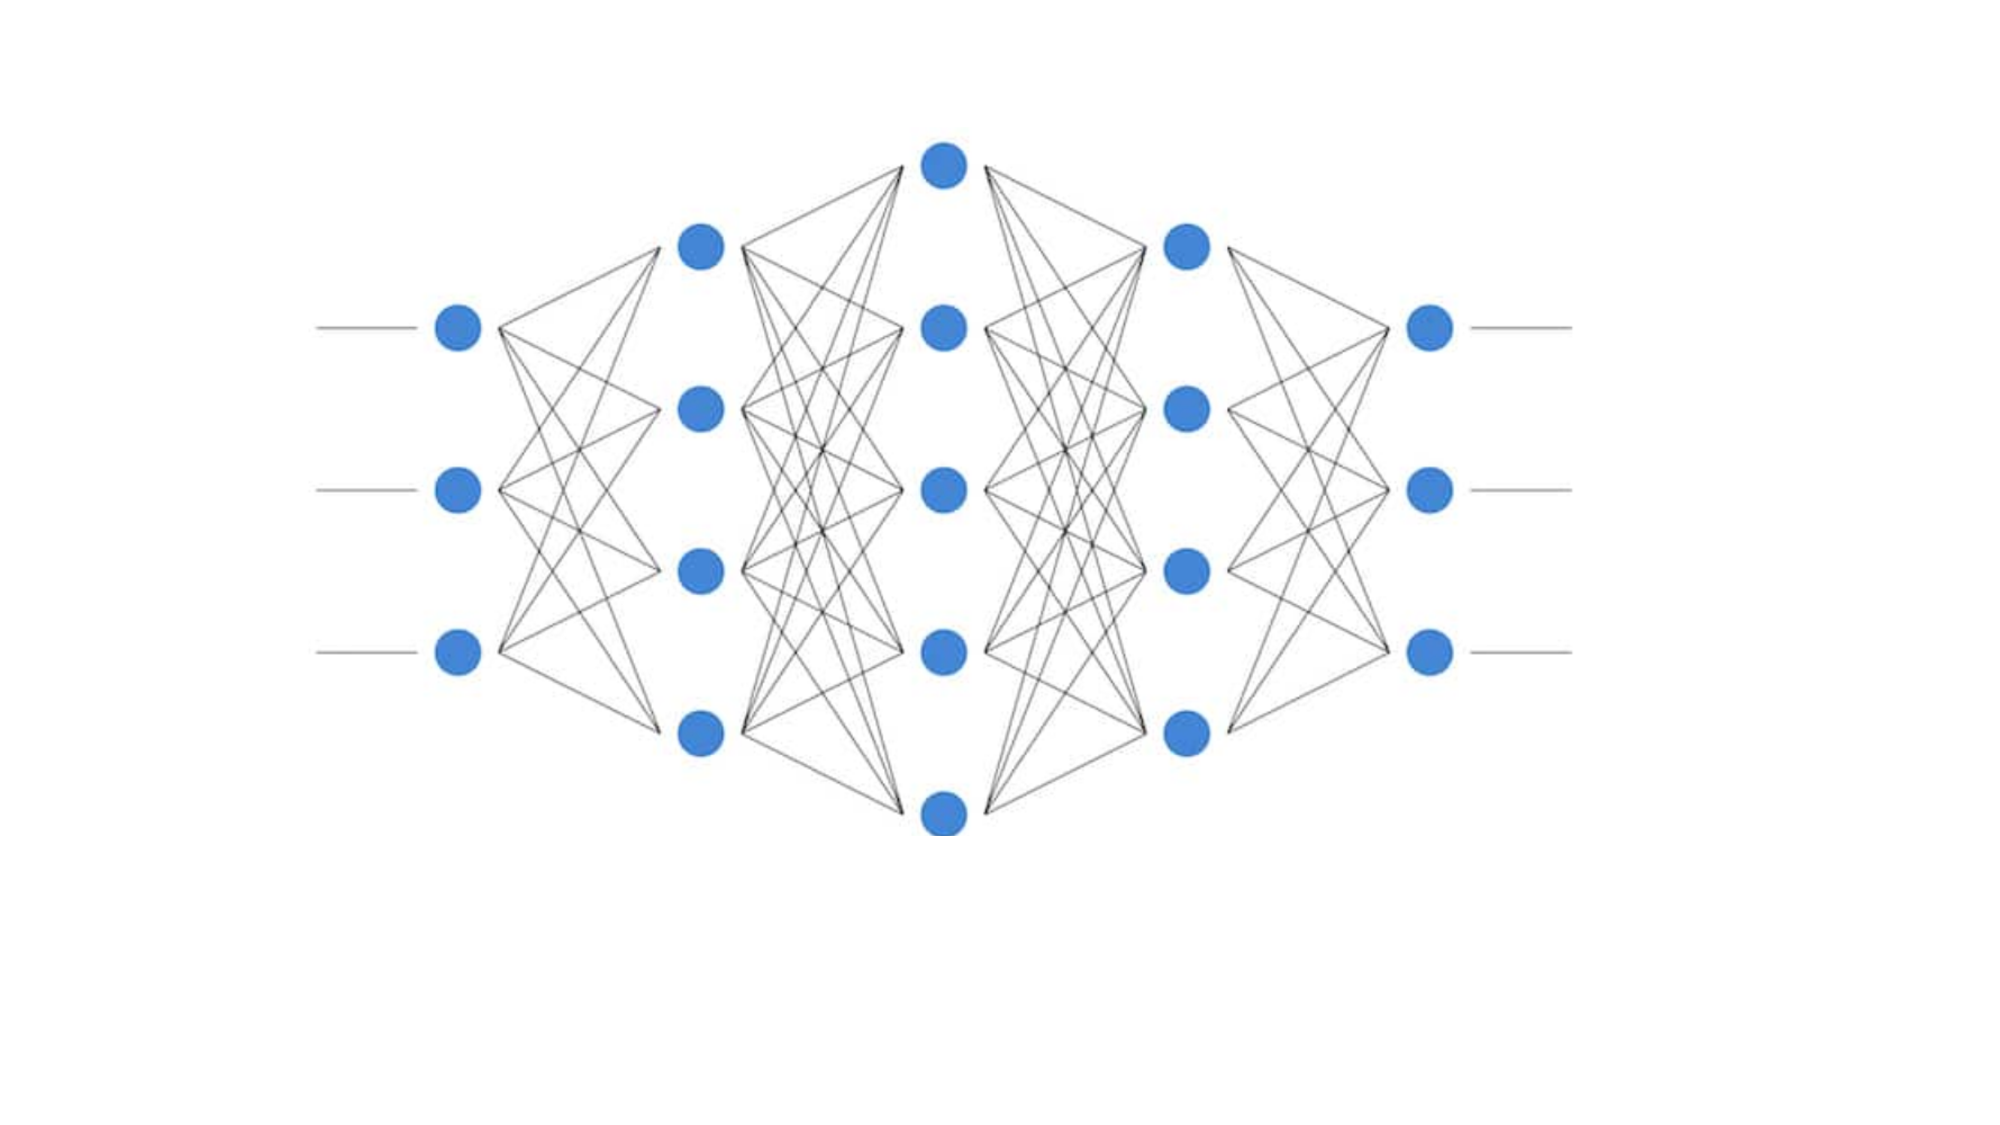
\includegraphics[width=0.8\linewidth]{example_figure.pdf}
\caption{here is an example figure }
\label{example_figure_label}
\end{figure}

%%%%%%%%%%%%

\subsection{Tables}

All tables must be centered, neat, clean and legible.  The table number and
title always appear before the table.  See Table~\ref{sample-table}.

Place one line space before the table title, one line space after the
table title, and one line space after the table. The table title must
be lower case (except for first word and proper nouns); tables are
numbered consecutively.

Note that publication-quality tables \emph{do not contain vertical rules.} We
strongly suggest the use of the \verb+booktabs+ package, which allows for
typesetting high-quality, professional tables:
\begin{center}
  \url{https://www.ctan.org/pkg/booktabs}
\end{center}
This package was used to typeset Table~\ref{sample-table}.

\begin{table}
  \caption{Sample table title}
  \label{sample-table}
  \centering
  \begin{tabular}{lll}
    \toprule
    \multicolumn{2}{c}{Part}                   \\
    \cmidrule(r){1-2}
    Name     & Description     & Size ($\mu$m) \\
    \midrule
    Dendrite & Input terminal  & $\sim$100     \\
    Axon     & Output terminal & $\sim$10      \\
    Soma     & Cell body       & up to $10^6$  \\
    \bottomrule
  \end{tabular}
\end{table}


\begin{itemize}

\item This is how you make a list of things

\end{itemize}

\subsubsection*{Acknowledgments}

Use unnumbered third level headings for the acknowledgments. All acknowledgments
go at the end of the paper. Do not include acknowledgments in the anonymized
submission, only in the final paper.




%%%%%%%%%%%%%%%%%%%%%%%%%%%%%%%%%%%%%%%
%Bibliography

\begin{thebibliography}{99}

\bibitem{Lecun15} Y. LeCun, Y. Bengio and G. Hinton, ``Deep Learning," Nature {\bf 521}, 436--444 (2015).

 \end{thebibliography}
 

\end{document}



%%%%%%%%%%%%%%%%%%%%%%
%%Experimental results table, thin smear, with center LED
%\begin{table}[b]
%  \caption{DP-CNN classification of {\it P. falciparum} infection, thin smear, with center LED}
%  \label{sample-table}
%  \centering
%  \begin{tabular}{lllllllll}
%    \toprule
%   \multicolumn{2}{c}{ }     & \multicolumn{7}{c}{Illumination Type \& Classification Score}               \\
%    \cmidrule{3-9}
%    Data & Value & Center & Off-axis & DPC & All & Random & PC Ring & Optim.   \\
%    \midrule
%    %Red-only & Average & 0.829 & 0.713 & 0.708 & 0.710 & 0.724 & 0.845 & 0.862 \\
%     %& Majority & 0.849 & 0.722 & 0.723 & 0.722 & 0.759 & 0.854 & {\bf 0.894} \\
%     %& STD & 0.013 & 0.015 & 0.011 & 0.012 & 0.046 & 0.011 & 0.018  \\
%    \midrule
%    %This was the second run with the PC Ring data, I messed up the first run
%     Red-only & Average & 0.839 & 0.772 & 0.708 & 0.781 & 0.762 & 0.881 & 0.890 \\
%     & Majority & 0.845 & 0.796 & 0.715 & 0.797 & 0.797 & 0.891 & {\bf 0.906} \\
%     & STD & 0.017 & 0.016 & 0.011 & 0.018 & 0.045 & 0.011 & 0.011  \\
%    \midrule
%    Green-only & Average & 0.873 & 0.736 & 0.717 & 0.727 & 0.772 & 0.900 & 0.897 \\
%     & Majority & 0.885 & 0.739 & 0.721 & 0.755 & 0.834 & 0.911 & {\bf 0.915}  \\
%     & STD & 0.022 & 0.010 & 0.017 & 0.012 & 0.046 & 0.011 & 0.016 \\
%    \midrule
%    Blue-only & Average & 0.869 & 0.745 & 0.792 & 0.753 & 0.813 & 0.881 & 0.887 \\
%     & Majority & 0.875 & 0.761 & 0.816 & 0.766 & 0.875 & 0.895 & {\bf 0.922}  \\
%     & STD & 0.012 & 0.015 & 0.006 & 0.014 & 0.032 & 0.014 & 0.017 \\
%     \midrule
%     RGB, cent init & Average & 0.917 & 0.779 & 0.750 & 0.727 & 0.785 & 0.879 & 0.928 \\
%     & Majority & 0.935 & 0.799 & 0.770 & 0.744 & 0.833 & 0.911 &{\bf 0.946}  \\
%     & STD & 0.005 & 0.006 & 0.009 & 0.022 & 0.028 & 0.011 & 0.007 \\
%    \bottomrule
%  \end{tabular}
%\end{table}



%%%%%%%%%%%%%%%%%%%%%
%Experimental results table, thin smear, with center LED
%NOTE 11/7/18: This table is before adding the PC-ring results, in which case I took both the 
%PC Ring score from the new run, and the optimized case score from the new one
% The rest of the scores, including the center score, did not change at all really
%\begin{table}[b]
%  \caption{DP-CNN classification of {\it P. falciparum} infection, thin smear, with center LED}
%  \label{sample-table}
%  \centering
%  \begin{tabular}{llllllll}
%    \toprule
%   \multicolumn{2}{c}{ }     & \multicolumn{6}{c}{Illumination Type \& Classification Score}               \\
%    \cmidrule{3-8}
%    Data & Value & Center & Off-axis & DPC & All & Random & Optim.   \\
%    \midrule
%    Red-only & Average & 0.829 & 0.713 & 0.708 & 0.710 & 0.724 & {\bf 0.852} \\
%     & Majority & 0.849 & 0.722 & 0.723 & 0.722 & 0.759 & {\bf 0.868} \\
%     & STD & 0.013 & 0.015 & 0.011 & 0.012 & 0.046 & 0.016  \\
%    \midrule
%    Green-only & Average & 0.873 & 0.736 & 0.717 & 0.727 & 0.772 & {\bf 0.883} \\
%     & Majority & 0.885 & 0.739 & 0.721 & 0.755 & 0.834 & {\bf 0.900}  \\
%     & STD & 0.022 & 0.010 & 0.017 & 0.012 & 0.046 & 0.016 \\
%    \midrule
%    Blue-only & Average & 0.869 & 0.745 & 0.792 & 0.753 & 0.813 & {\bf 0.883} \\
%     & Majority & 0.875 & 0.761 & 0.816 & 0.766 & 0.875 & {\bf 0.910}  \\
%     & STD & 0.012 & 0.015 & 0.006 & 0.014 & 0.032 & 0.023 \\
%%    \midrule
%%     RGB 3K, rand init & Average & 0.875 & 0.747 & 0.739 & 0.713 & 0.766 & 0.877 \\
%%     & Majority & 0.893 & 0.752 & 0.748 & 0.724 & 0.830 & 0.901  \\
%%     & STD & 0.017 & 0.022 & 0.016 & 0.020 & 0.032 & 0.018 \\
%     \midrule
%     RGB, cent init & Average & 0.918 & 0.779 & 0.750 & 0.727 & 0.785 & {\bf 0.930} \\
%     & Majority & 0.933 & 0.799 & 0.770 & 0.744 & 0.833 & {\bf 0.941}  \\
%     & STD & 0.005 & 0.006 & 0.009 & 0.022 & 0.028 & 0.007 \\
%    \bottomrule
%  \end{tabular}
%\end{table}
